\begin{figure}[bt!]
  \begin{center}
    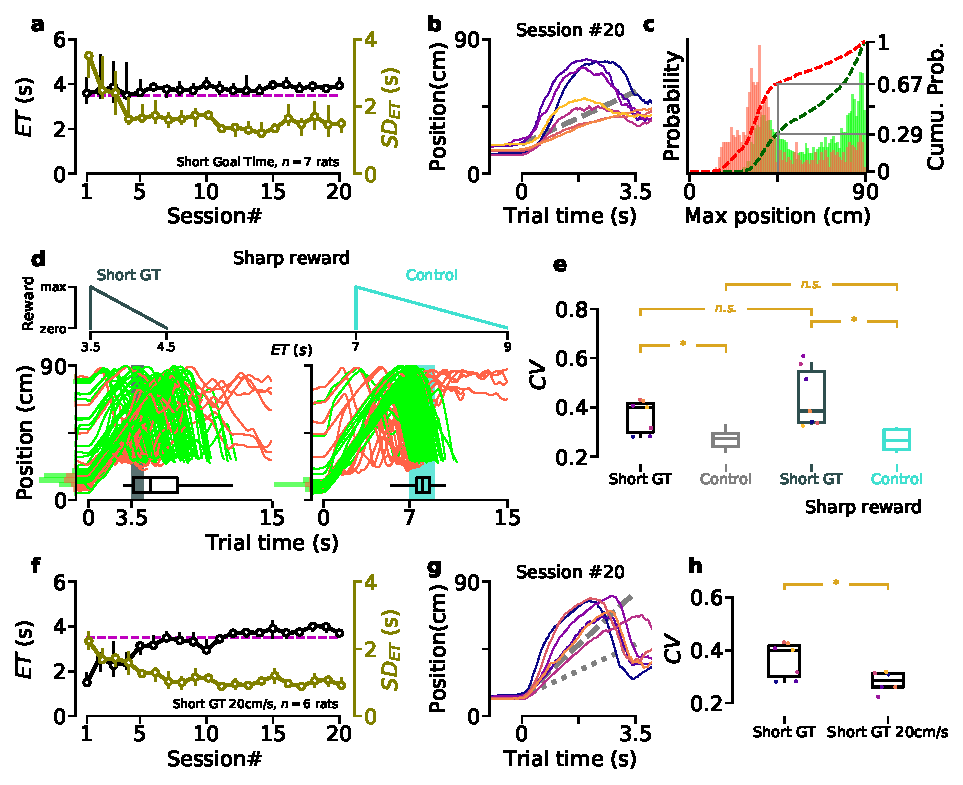
\includegraphics[width=.8\linewidth]{ch-time/figures/ShortGT-SharpTrd.pdf}
    \caption[Short GT and sharp conditions]
    {\textbf{Decreased temporal accuracy when the goal time is shortened.}
    \textbf{a)}
    Median entrance time~($ET$) during training.
    The dashed magenta line shows the goal time~($GT=3.5$~s).
    The right y-axis shows standard deviation~($SD$) of $ET$.
    \textbf{b)}
    Median trajectory of "short GT" animals after training.
    Colored lines indicate performance of individual animals.
    Dashed line's slope shows the treadmill speed (10~cm/s).
    \textbf{c)}
    PDF of the maximum position reached by short GT animals before $ET$ for correct (green) and incorrect (red) trials.
    Dashed lines represent cumulative distribution functions (right y-axis).
    Data collected from session~\#~$\geq15$.
    \textbf{d)} 
    Sharp reward condition applied to short GT and control experiments.
    \textit{Top}: reward profiles in the sharp condition.
    \textit{Bottom}: trajectories of 2 illustrative sessions after training in sharp condition (\textit{left}, short GT; \textit{right}, control).
    Highlighted areas indicate the reward window.
    \textbf{e)}
    Coefficient of variation~($CV$) for short GT and control experiments with normal (first two boxes), and sharp (last two boxes) reward profiles.
    Data collected and averaged once performance plateaued (after session~\#15 for short GT, between session~\#20 to~\#30 for control, and last 5 sessions for the sharp condition experiments).
    Short GT vs. Control: $p<0.0001$ (permutation test, see \nameref{methods});
    Sharp short GT vs. Sharp control: $p<0.0001$ (permutation test);
    Short GT vs. Sharp short GT: Non significant (non-parametric paired comparison); 
    Control vs. Sharp control: $p=0.79$ (permutation test).
    \textbf{f)}
    Similar to panel~a, for another group of animals that were trained to wait for 3.5~s while the speed of the treadmill was 20~cm/s.
    \textbf{g)}
    Similar to panel~b, for animals trained in short goal time 20~cm/s condition (panel~f).
    Dashed line's slope shows the treadmill speed (20~cm/s).
    Dotted line's slope indicates control treadmill speed (10~cm/s).
    \textbf{h)}
    $CV$ for short GT and short GT 20~cm/s conditions (same colors as in panel~b,g).
    Data collected and averaged once performance plateaued (after session~\#15).
    Short GT vs. Short GT 20~cm/s: Asterisk indicates significant difference (10,000 resamples with replacement, see \nameref{methods}).
    }
    \label{fig:time:shortSharp}
  \end{center}
\end{figure}
